\section{Input Parsing}

The following diagram provides a high-level overview of the steps of the input parsing process:

\begin{figure}[htbp]
\centerline{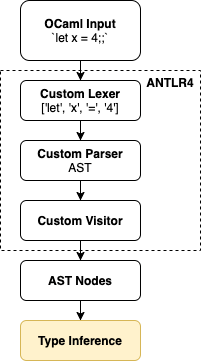
\includegraphics[scale=.6]{images/parse-process-diagram.png}}
\caption{Overview of input parsing process}
\label{fig}
\end{figure}

\subsection{Use of ANTLR4ts}
ANTLR4ts is a very useful open-source tool that generates lexer, parser and visitor files based on the specified supported grammar for a language. We used this tool in order to bypass the need for manual parsing, and focus more on the core type inference algorithm. In the process of using ANTLR4ts, we encountered the following challenges and design decisions:
\begin{enumerate}
    \item Translating OCaml grammar in Backus–Naur Form (BNF) to ANTLR4 g4 format
    \item Deciding whether to use Visitors or Listeners to traverse the AST
\end{enumerate}
  
\subsection{Translation of OCaml grammar from BNF to ANTLR4 g4 format}
This section of the project introduced some early challenges as we got to grips with understanding OCaml expressions as specified in the BNF grammar, as well as understanding how the ANTLR4 g4 format works. One challenge we faced was handling cases where we do not want to support the 'default' left recursion, such as mathematical expressions that have to respect operator precedence. Another challenge was related to the ordering of rules in the g4 file itself, where rules appearing early in the file were causing unintended consequences in the application of rules that appear later in the file. \\

In the end, we came up with two versions of the grammar - a complete one as a community contribution to the ANTLR4 repository, as well as a scoped down version for use in our type checker.
  
\subsection{Deciding between Visitors and Listeners}
ANTLR4 offers two patterns for traversing the AST generated from parsing - Visitors and Listeners. Both these mechanisms use depth-first search to traverse the tree, but they have the following differences: 
\begin{enumerate}
    \item Listener methods are independently and automatically called by a walker object provided by ANTLR, while visitor methods make use of explicit visit calls in order to visit children
    \item Listener methods don't return a value, while visitor methods can return any custom type
    \item The Listener pattern uses an explicit stack allocated on the heap, while the Visitor pattern uses the call stack to manage tree traversals
\end{enumerate}
 After analyzing these two patterns, we decided to go with the Visitor pattern primarily because it allows us to explicitly decide which sub-trees to visit. Furthermore, it allows us to return custom ASTNodes from the traversal of such trees. As a result, we enjoy better control in managing and manipulating the AST. However, we accept that this comes at the cost of potential StackOverFlow exceptions in non-tail recursive cases that generate deeply nested ASTs.
 
\subsection{AST Nodes}
Following traversing the AST using visitors, we then generate ASTNodes of various types to encapsulate the nature of the expression being type-checked. One of the key ASTNodes we implemented is the Let node, as defined below:

\scriptsize
\begin{Verbatim}[tabsize=4]
export class Let implements AstNode {
    constructor(public variable: Id, public value: AstNode, public body: AstNode) { }
    toString() { return {`(let {this.variable} = {this.value} in {this.body})`} }
}
\end{Verbatim}

\normalsize

These nodes containing additional labels and context are then used by the type inference algorithm.
